\documentclass{beamer}

\newcommand\tab[1][1cm]{\hspace*{#1}}
\usepackage[spanish]{babel}
\usepackage[utf8]{inputenc}
\usepackage{bussproofs}
\usepackage{url}
\usepackage[document]{ragged2e}

\DeclareOptionBeamer{compress}{\beamer@compresstrue}
\ProcessOptionsBeamer

\mode<presentation>

\useoutertheme[footline=authortitle]{miniframes}
\useinnertheme{circles}
\usecolortheme{whale}
\usecolortheme{orchid}

\definecolor{beamer@blendedblue}{rgb}{0.137,0.466,0.741}

\setbeamercolor{structure}{fg=beamer@blendedblue}
\setbeamercolor{titlelike}{parent=structure}
\setbeamercolor{frametitle}{fg=black}
\setbeamercolor{title}{fg=black}
\setbeamercolor{item}{fg=black}

\setbeamertemplate{bibliography item}[text]

\mode
<all>

\title[]{Introducción a Hyperledyer Fabric}
\subtitle{Fundamentos de blockchains}
\author{René Dávila - Jorge Solano}
\date{ }

\AtBeginSection[] { 
	\begin{frame} 
		\frametitle{Índice}
		\tableofcontents[currentsection]
	\end{frame}
}
\AtBeginSubsection[] { 
	\begin{frame}
		\frametitle{Índice}
		\tableofcontents[currentsection, currentsubsection]
	\end{frame}
}

\setbeamertemplate{navigation symbols}{}

\begin{document}
	\frame{\titlepage}
	\EnableBpAbbreviations

	\section{Introducción}
	\begin{frame}
		\begin{block}{Hyperledger project}
			La Linux Foundation se caracteriza por nutrir proyectos \textbf{open source} de \textbf{open governance} que genera comunidades sostenibles fuertes y ecosistemas prósperos.\\
			\vspace{4mm}
			\textbf{Linux Foundation} creó el projecto \textbf{Hyperledger} en 2015 para avanzar en la industria de la tecnología de blockchain.
		\end{block}
	\end{frame}

	\begin{frame}
		\begin{block}{Hyperledger project}
			\textbf{Hiperledger Fabric} es uno de los \textbf{proyectos de blockchain en Hyperledger}, el cual (como otros) es un ledger que utiliza smart contracts y donde los participantes manejan las transacciones.
		\end{block}
	\end{frame}

	\subsection{Blockchain}
	\begin{frame}
		\frametitle{Blockchain}
		En términos generales, una \textbf{blockchain} se podría considerar como un \textbf{libro mayor} en el área contable \textbf{(ledger)}. Es un lugar donde se llevan a cabo transacciones inmutables dentro de una red de nodos distribuida.\\
		\vspace{4mm}
		Cada uno de estos \textbf{nodos} mantiene una \textbf{copia del libro} mayor aplicando transacciones que han sido validadas mediante el protocolo de consenso, agrupadas en bloques que incluyen un hash que permite enlazar cada bloque con su bloque anterior.
	\end{frame}
	
	\subsection{Criptomonedas}
	\begin{frame}
		\frametitle{Criptomonedas}
		La aplicación más reconocida de blockchain es la criptomoneda \textbf{Bitcoin}.\\
		\vspace{4mm}
		\textbf{Ethereum} es una criptomoneda alternativa, la cual integra muchas características de Bitcoin, pero agrega contratos inteligentes (smart contracts) con el fin de crear una plataforma para aplicaciones distribuidas.
	\end{frame}
	
	\begin{frame}
		Tanto \textbf{Bitcoin} como \textbf{Ethereum} caen en la clasificación de blockchain, las cuales clasificaremos como tecnologías de \textbf{blockchain públicas y sin permiso}. Básicamente, son redes públicas, abiertas a cualquiera, donde los participantes interactúan de manera anónima.
	\end{frame}

	\begin{frame}
		Sin embargo, en muchos casos de \textbf{uso empresarial} la \textbf{identidad} de los participantes es un \textbf{requisito indispensable}, como por ejemplo en una transacción financiera, donde las regulaciones el Know Your Customer (KYC) y el Anti-Money Laundering (AML) deben seguirse de manera puntual.
	\end{frame}
	
	\begin{frame}
		Para el uso empresarial de blockchain se deben considerar los siguientes requerimientos:
		
		\begin{itemize}
			\item Cada participante debe identificarse y ser identificable.
			\item Las redes deben estar autorizadas.
			\item Alto rendimiento durante las transacciones.
			\item Baja latencia en la confirmación de transacción.
			\item Privacidad y confidencialidad de las transacciones y de la información de las transacciones.
		\end{itemize}
	\end{frame}
	
	\section{Hyperledger Fabric v2.0}
	
	\begin{frame}
		\begin{block}{Hyperledger Fabric v2.0}
			Hyperledger Fabric es una plataforma \textbf{open source} de grado \textbf{empresarial}, que permite manejar un tecnología distribuida de ledger.\\
			\vspace{4mm}
			Tiene algunas \textbf{capacidades claves} diferentes con respecto a otros ledger distribuidos o a otras plataformas de blockchain.
		\end{block}
	\end{frame}

	\subsection{Componentes y características}
	
	\begin{frame}
		\frametitle{Private and permissioned}
		\textbf{Hiperledger Fabric} destaca por sobre otros sistemas de blockchain porque \textbf{es privada y autorizada}, esto es, los miembros de la red se registran a través de un Membership Service Provider (MSP) de confianza.\\
	\end{frame}

	\begin{frame}
		Entonces, si los participantes no pueden confiar completamente uno en el otro (por ejemplo, si son competidores en la misma industria), la red puede operar bajo el modelo de gobierno  basado en la confianza que existe entre los participantes, como lo es un acuerdo legal o un marco de referencia para manejar disputas.
	\end{frame}
	
	\begin{frame}
		\frametitle{Pluggable}
		\textbf{Hyperledger Fabric} ofrece varias \textbf{opciones enchufables}. La información del ledger puede guardarse en múltiples formatos, los mecanismos de consenso se pueden intercambiar y se pueden tener diferentes Provedores de Servicio de Membresía (MSP).\\
		\vspace{4mm}
		Esto permite que la plataforma sea personalizada y se ajuste a casos de uso y modelos confiables particulares.
	\end{frame}

	\begin{frame}	
		Por ejemplo, dentro de una empresa o en una empresa operada por una autoridad de confianza, el protocolo de consenso tolerante a fallas bizantinas podría considerarse innecesario y hasta excesivo, en su lugar se podría pensar que el protocolo de consenso tolerante a fallas sería más apropiado.
	\end{frame}
	
	\begin{frame}
		\frametitle{Channels}
		\textbf{Hyperledger Fabric} ofrece la posibilidad de crear \textbf{canales}, lo que permite que un grupo de participantes tenga su propio ledger de transacciones.\\
		\vspace{4mm}
		Esta capacidad es importante en redes donde algunos participantes pueden ser competidores y no quieren que cada transacción (pe, una oferta especial en un producto) sea conocida por cada participante.
	\end{frame}

	\begin{frame}
		\frametitle{Shared Ledger}
		El ledger de \textbf{Hyperledger Fabric} comprende dos componentes: el \textbf{world state} y la \textbf{transaction log}. Cada participante tiene una copia del ledger de cada red a la que pertenece.\\
		\vspace{4mm}
		El world state representa la base de datos del ledger. La transaction log guarda la historia actualizada del world state. El ledger es, entonces, la combinación de la BD del world state y la historia de la transaction log.
	\end{frame}
	
	\begin{frame}
		\frametitle{Smart contracts}
		Los \textbf{smart contracts} de \textbf{Hyperledger Fabric} están escritos en chaincode y son invocados por una aplicación externa a la blockchain. En la mayoría de los casos, el chaincode interactúa directamente con la base de datos del ledger (world state) y no con la log transaction.\\
		\vspace{4mm}
		El \textbf{chaincode} puede ser implementado \textbf{en lenguajes de programación de uso general} (como Java, Go y Node.js), por lo que no se requiere aprender un lenguaje de dominio específico.\\
	\end{frame}

	\begin{frame}
		\frametitle{Privacy}
		\textbf{Hyperledger Fabric} permite crear tanto redes donde la \textbf{privacidad} (utilizando canales) es un requerimiento operacional clave, así como redes abiertas.
	\end{frame}
	
	\begin{frame}
		\frametitle{Consensus}
		\textbf{Hyperledger Fabric} está diseñado para permitir que las redes elijan el \textbf{mecanismo de consenso} que mejor se acomode a la relación que existe entre los participantes.
	\end{frame}
		
	\begin{frame}
		\textbf{Fabric} puede aprovechar los protocolos de consenso que \textbf{no requieren criptomonedas} nativas para incentivar la minería o la ejecución de contratos inteligentes. Evitar las criptomonedas \textbf{reduce} de manera significativa \textbf{el riesgo o los vectores de ataque}.\\
		\vspace{4mm}
		Además, la ausencia de las operaciones de minería criptográfica permite que la plataforma se pueda desplegar con prácticamente el mismo costo operacional que cualquier otro sistema distribuido. 
	\end{frame}
	
	\section{Instalación de Hyperledger Fabric v2.0}
	
	\begin{frame}
		Para poder instalar \textbf{Hyperledger Fabric} es necesario tener ciertas herramientas ya instaladas donde se va a ejecutar. Entonces, primero hay que verificar o instalar los \textbf{prerrequisitos de instalación}.
	\end{frame}
	
	\subsection{Prerrequisitos de instalación}
	
	\begin{frame}
		\frametitle{Prerrequisitos de instalación}
		Para poder desarrollar aplicaciones con Hyperledger Fabric se deben tener instaladas las siguientes herramientas:
		\begin{itemize}
			\item Git
			\item curl
			\item Docker y Docker Compose (versión 17.06.2-ce o superior)
			\item Go
			\item Node.js y NPM
			\item Python
		\end{itemize}
	\end{frame}
	
	\begin{frame}
		\frametitle{Git (\url{https://git-scm.com/downloads})}
		\textbf{Git} es un controlador de versiones distribuido, gratuito y de código abierto diseñado para manerjar proyectos de diferente tamaño con eficiencia.
		\begin{figure}[h]
			
\includegraphics[scale=.3]{git}
			\centering
		\end{figure}
	\end{frame}

	\begin{frame}
		\frametitle{curl (\url{https://curl.haxx.se/download.html})}
		\textbf{curl} (Client URL) es una biblioteca y una herramienta de línea de comandos que permite transferir datos a través de diferentes protocolos.
		\begin{figure}[h]
			
\includegraphics[scale=.3]{curl}
			\centering
		\end{figure}
	\end{frame}

	\begin{frame}
		\frametitle{Docker (\url{https://www.docker.com/get-docker})}
		\textbf{Docker} es un contenedor de aplicaciones. Un contenedor es una unidad estándar de software que empaqueta código y todas sus dependencias para que la aplicación se ejecute de manera confiable y rápida en cualquier entorno de computadora.
		\begin{figure}[h]
			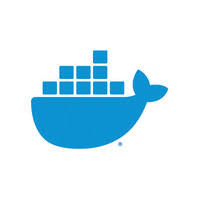
\includegraphics[scale=.3]{docker}
			\centering
		\end{figure}
	\end{frame}
	
	\begin{frame}
		\frametitle{Docker Compose (\url{https://docs.docker.com/compose/install/})}
		\textbf{Compose} es una herramienta para definir y ejecutar múltiples contenedores de aplicaciones Docker. Docker-compose ya está incluida en Docker Desktop.
		\begin{figure}[h]
			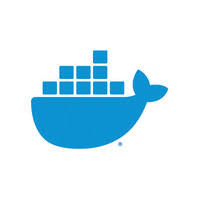
\includegraphics[scale=.3]{docker}
			\centering
		\end{figure}
	\end{frame}

	\begin{frame}
		\frametitle{Go (\url{https://golang.org/dl/})}
		\textbf{Go} es un lenguaje de programación de código abierto que permite crear software simple, confiable y eficiente.
		\begin{figure}[h]
			
\includegraphics[scale=.3]{go}
			\centering
		\end{figure}
	\end{frame}
	
	\begin{frame}
		\frametitle{Node.js (\url{https://nodejs.org/en/download/})}
		\textbf{Node.js} es un entorno de ejecución de JavaScript, de código abierto y multiplataforma, que permite ejecutar código JavaScript fuera de un navegador web.
		\begin{figure}[h]
			
\includegraphics[scale=.3]{nodejs}
			\centering
		\end{figure}
	\end{frame}
	
	\begin{frame}
		\frametitle{NPM (\url{https://www.npmjs.com/get-npm})}
		\textbf{NPM} es un administrador de paquetes para el lenguaje de programación JavaScript. Es el administrador de paquetes por defecto de Node.js.
		\begin{figure}[h]
			
\includegraphics[scale=.3]{npm}
			\centering
		\end{figure}
	\end{frame}
	
	\begin{frame}
		\frametitle{Python (\url{https://www.python.org/downloads/})}
		\textbf{Python} lenguaje de programación interpretado, de alto nivel y de propósito general.
		\begin{figure}[h]
			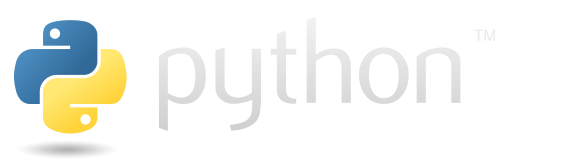
\includegraphics[scale=.3]{python}
			\centering
		\end{figure}
	\end{frame}

	\subsection{Instalación}
	
	\begin{frame}
		\frametitle{Instalación}
		Una vez instalados los prerrequisitos, se cuenta con el ambiente listo para descargar e instalar Hyperledger Fabric. Actualmente el proyecto no cuenta con un instalador de los binarios de Fabric, pero los ejemplos que se descargan poseen scripts de ejecución.
	\end{frame}
	
	\begin{frame}
		\frametitle{Instalación}
		Para la instalación hay que ubicarse en la ruta donde se van a descargar los ejemplos y binarios de Fabric, hay que descargar los binarios y las imágenes:\\
		\begin{center}
			\setlength{\fboxrule}{1mm}
			\setlength{\fboxsep}{3mm}
			\framebox[9cm][c]{
					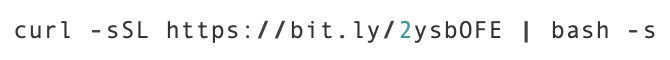
\includegraphics[scale=.7]{install_01}
			}
		\end{center}
	\end{frame}

	\begin{frame}
		\frametitle{Instalación}
		La instrucción anterior descarga y descomprime los binarios requeridos y específicos para la plataforma y los guarda en el repositorio (\textbf{fabric-samples}) dentro de la carpeta \textbf{bin}.
		\begin{figure}[h]
			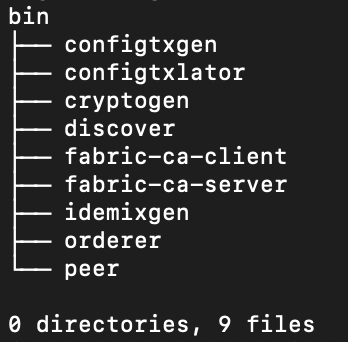
\includegraphics[scale=.5]{install_02}
			\centering
		\end{figure}
	\end{frame}
	
	\begin{frame}
		\frametitle{Instalación}
		Por último, hay que mapear la carpeta bin al PATH del sistema. Aquí es importante comentar que también go y go/bin deben estar en el PATH.\\
		\begin{center}
			\setlength{\fboxrule}{1mm}
			\setlength{\fboxsep}{3mm}
			\framebox[9cm][c]{
				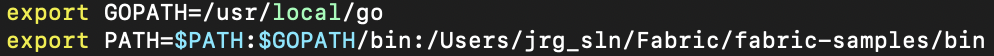
\includegraphics[scale=.5]{install_03}
			}
		\end{center}
	\end{frame}
	
	\section{Hyperledger en acción}
	
	\begin{frame}
		\frametitle{Let's do it!}
		Una vez descargado Hyperledger Fabric ya es posible desplegar alguno de los proyectos que se descargaron.\\
		\vspace{4mm}
		En realidad, se descargaron imágenes y ejemplos Docker, esto es, contenedores con aplicaciones precargadas, las cuales se guardaron en la carpeta \textbf{fabric-samples}.
	\end{frame}

	\begin{frame}
		\frametitle{Let's do it!}
		Vamos a trabajar con la red test-network que está dentro de la carpeta fabric-samples (cd fabric-samples/test-network).\\
		\vspace{4mm}
		En esa carpeta se encuentra el script \textit{network.sh}, el cual levanta una red Fabric utilizando las imágenes Docker descargadas. Para ver las opciones del script se puede ejecutar \textit{network.sh -h}
	\end{frame}
	
	\section{Referencias}
	
	\begin{frame} [allowframebreaks]
		\frametitle{Referencias}
		\nocite{hyper, docker}
		\bibliographystyle{plain}
		\bibliography{biblio}
	\end{frame}
\end{document}